\documentclass[12pt,a4paper,titlepage]{article}

\usepackage[T1]{fontenc}
\usepackage[polish]{babel}
\usepackage[utf8]{inputenc}
\usepackage{lmodern}
\usepackage{graphicx}
\selectlanguage{polish}

\setlength{\parindent}{5mm} %ustawi rozmiar wcie˛cia na pocza˛tku kaz˙dego akapitu na 0mm,
\setlength{\parskip}{4mm}	%

\title{Sprawozdanie z ćwiczenia laboratoryjnego}
\date{2014}
\author{Tomasz Mikołajewski }

\begin{document}
\maketitle
\pagestyle{empty}
%\pagestyle{headings}
\tableofcontents

\section{Wprowadzenie}
Niniejszy dokument powstał w ramach przedmiotu Projektowanie Algorytmów i Metod Sztucznej Inteligencji. Jest on rezultatem przeprowadzonych ćwiczeń w laboratorium oraz pracy wykonanej w domu.


Ćwiczenie polegało na przeprowadzeniu analizy zapisu do struktur stosu oraz kolejki. Struktury zostały stworzone w oparciu o tablicę oraz listę. Podczas wykonywania czynności przepisywania liczony był czas wykonania operacji. Testowanie powtarzano wielokrotnie, aby uzyskać ilość danych pozwalającą na wyznaczenie przybliżonej funkcji opisującej złożoność algorytmu. 

\section{Kod programu}
Program został oparty o wcześniej stworzone pliki zawierające kod potrzebny do wykonania \textit {benchmark-u} podprogramu, czyli określenia czasu jaki potrzebny jest na jego wykonanie. Główny program zawiera funkcję otwierającą pliki z danymi oraz zapisującą rezultat operacji do pliku. Zdecydowanie ułatwia to prace przy analizie zadanego algorytmu.

Struktury, które były testowane to:
\begin{itemize}
\item stos stworzony za pomocą tabeli
\item stos stworzony za pomocą listy
\item kolejka stworzona za pomocą tabeli
\item kolejka stworzona za pomocą listy
\end{itemize}


Dodatkowo algorytmy zrealizowane na tablicy posiadały dwie możliwości kompilacji kodu: tablica powiększająca się za każdym razem oraz tablica powiększająca się razy 2.

\section{Pomiary}
Pomiary zostały przeprowadzone na dużych plikach zawierających zmienne typu \textit {int}. Każdy z algorytmów był testowany dla co najmniej 5 różnych rozmiarach problemów powtórzonych dla dwóch różnych plików. Aby otrzymać rzetelny pomiar, każdy z testów był przeprowadzony 3-krotnie. Oznacza to iż każdy z algorytmów był testowany co najmniej 30 razy. 

\section{Wyniki pomiarów}
Po przeprowadzeniu serii pomiarów otrzymano wyniki przedstawione w tabelach. Na podstawie wyników utworzono wykresy zamieszczone poniżej.


\subsection{Stos stworzony na podstawie tablicy}
Grupa ta zawiera dwie podgrupy ze względu na rodzaj wykonywanego algorytmu.


\subsubsection{Powiększanie tablicy za każdym razem}
Metoda wykonująca większą ilość obliczeń.

\begin{center}
\begin {tabular}{|c|c|c|c|c|}\hline
Wielkosc & 1 & 2 & 3 & Średnia \\\hline
1000 &	0	&	0	 &	0,015 &	0,005 \\\hline 
1000 &	0	&	0,016 &	0	 &	0,0053 \\\hline 
3000 &	0,046 &	0,047 &	0,047 &	0,0467 \\\hline 
3000 &	0,047 &	0,063 &	0,047 &	0,0523 \\\hline 
5000 &	0,14 &	0,141 &	0,125 &	0,1353 \\\hline 
5000 &	0,141 &	0,141 &	0,125 &	0,1357 \\\hline 
10000 &	0,547 &	0,531 &	0,531 &	0,5363 \\\hline 
10000 &	0,531 &	0,547 &	0,547 &	0,5417 \\\hline 
30000 &	4,812 &	4,843 &	4,922 &	4,859 \\\hline 
30000 &	4,812 &	4,828 &	5,078 &	4,906 \\\hline 
50000 &	13,344 &	13,5 &	14,235 &	13,693 \\\hline 
50000 &	13,469 &	13,781 &	14,015 &	13,755 \\\hline 
100000 &	53,781 &	55,828 &	56,938 &	55,5157 \\\hline 
100000 &	54,391 &	55,719 &	64,75 &	58,2867 \\\hline
\end{tabular}
\end {center}
\begin{figure}[h]
\begin{center}
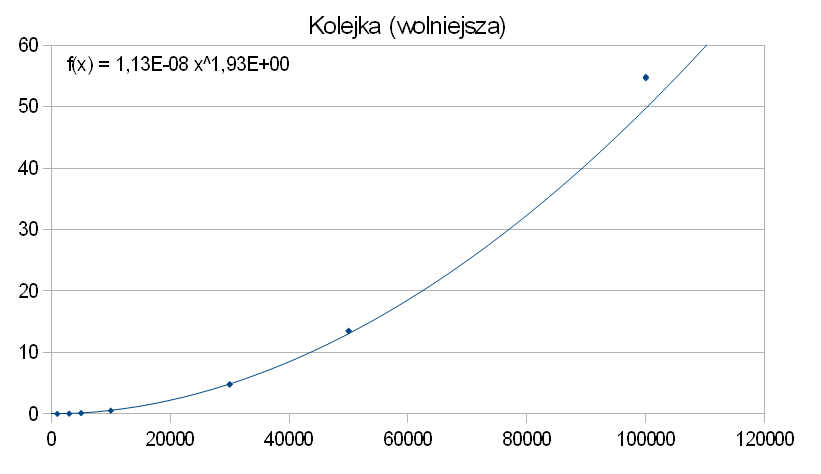
\includegraphics[scale=0.5]{kolejka_1.png}
\end{center}
\end{figure}

\newpage
\subsubsection{Powiększanie tablicy dwukrotnie}
Metoda wykonująca mniejszą ilość obliczeń.

\begin{center}
\begin {tabular}{|c|c|c|c|c|}\hline
Wielkosc & 1 & 2 & 3 & Średnia \\\hline
1100000&0,05&0,05&0,06&0,05 \\\hline 
100000&0,05&0,06&0,05&0,05 \\\hline 
500000&0,22&0,23&0,25&0,23 \\\hline 
500000&0,23&0,24&0,25&0,24 \\\hline 
1000000&2,03&2,14&2,08&2,08 \\\hline 
1000000&1,91&2,3&2,33&2,18 \\\hline 
5000000&6,42&6,67&6,81&6,64 \\\hline 
5000000&6&6,98&6,92&6,64 \\\hline 
10000000&13,09&13,88&14,36&13,78 \\\hline 
10000000&13,02&13,97&14,03&13,67 \\\hline 
\end{tabular}
\end {center}
\begin{figure}[h]
\begin{center}
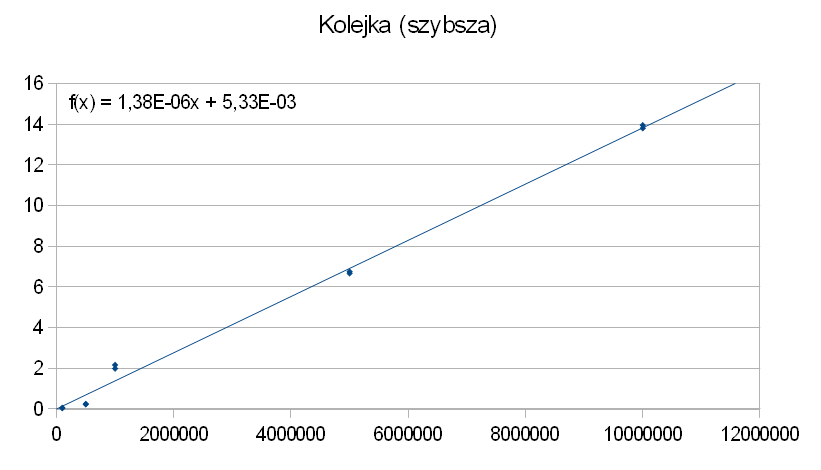
\includegraphics[scale=0.5]{kolejka_2.png}
\end{center}
\end{figure}

\newpage
\subsection{Kolejka stworzona na podstawie tablicy}
Grupa ta zawiera dwie podgrupy ze względu na rodzaj wykonywanego algorytmu.


\subsubsection{Powiększanie tablicy za każdym razem}
Metoda wykonująca większą ilość obliczeń.

\begin{center}
\begin {tabular}{|c|c|c|c|c|}\hline
Wielkosc & 1 & 2 & 3 & Średnia \\\hline
1000&0&0&0,015&0,005 \\\hline
1000&0&0,016&0&0,0053 \\\hline
3000&0,046&0,047&0,047&0,0467 \\\hline
3000&0,047&0,063&0,047&0,0523 \\\hline
5000&0,14&0,141&0,125&0,1353 \\\hline
5000&0,141&0,141&0,125&0,1357 \\\hline
10000&0,547&0,531&0,531&0,5363 \\\hline
10000&0,531&0,547&0,547&0,5416 \\\hline
30000&4,812&4,843&4,922&4,859 \\\hline
30000&4,812&4,828&5,078&4,906 \\\hline
50000&13,344&13,5&14,235&13,693 \\\hline
50000&13,469&13,781&14,015&13,755 \\\hline
100000&53,781&55,828&56,938&55,5156 \\\hline
100000&54,391&55,719&64,75&58,2866 \\\hline
\end{tabular}
\end {center}
\begin{figure}[h]
\begin{center}
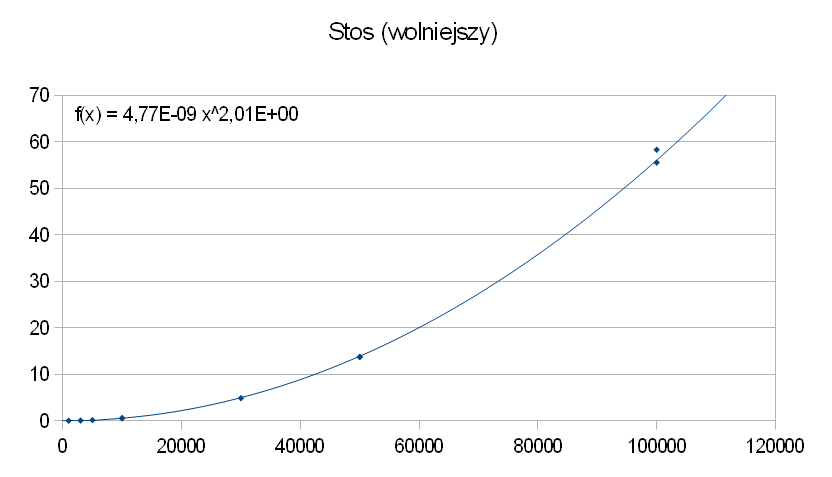
\includegraphics[scale=0.5]{stos_1.png}
\end{center}
\end{figure}

\newpage
\subsubsection{Powiększanie tablicy dwukrotnie}
Metoda wykonująca mniejszą ilość obliczeń.

\begin{center}
\begin {tabular}{|c|c|c|c|c|}\hline
Wielkosc & 1 & 2 & 3 & Średnia \\\hline
100000&0,047&0,047&0,062&0,052 \\\hline
100000&0,046&0,062&0,047&0,052 \\\hline
500000&0,219&0,234&0,25&0,234 \\\hline
500000&0,234&0,235&0,25&0,240 \\\hline
1000000&2,031&2,141&2,078&2,083 \\\hline
1000000&1,906&2,297&2,328&2,177 \\\hline
5000000&6,422&6,672&6,812&6,635 \\\hline
5000000&6&6,984&6,922&6,635 \\\hline
10000000&13,094&13,875&14,359&13,776 \\\hline
10000000&13,015&13,969&14,031&13,672 \\\hline
\end{tabular}
\end {center}
\begin{figure}[h]
\begin{center}
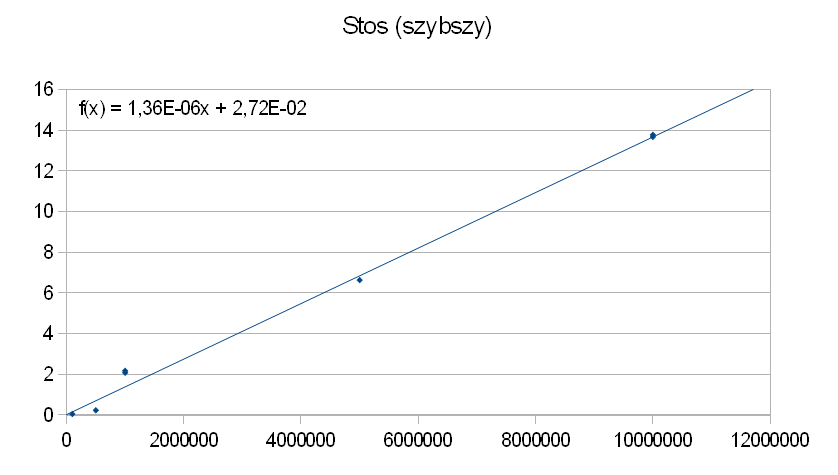
\includegraphics[scale=0.5]{stos_2.png}
\end{center}
\end{figure}

\newpage
\subsection{Stos stworzony na podstawie listy}
Klasa odpowiadająca za przechowywanie danych stworzona na podstawie klasy \textit{stack}. 
\begin{center}
\begin {tabular}{|c|c|c|c|c|}\hline
Wielkosc & 1 & 2 & 3 & Średnia \\\hline
100000&0&0&0&0 \\\hline
100000&0,015&0&0&0,005 \\\hline
500000&0,015&0,016&0,015&0,015 \\\hline
500000&0,031&0,016&0,031&0,026 \\\hline
1000000&0,047&0,031&0,047&0,042 \\\hline
1000000&0,062&0,046&0,031&0,046 \\\hline
5000000&0,219&0,203&0,344&0,255 \\\hline
5000000&0,219&0,219&0,234&0,224 \\\hline
10000000&0,671&0,391&0,484&0,515 \\\hline
10000000&0,515&0,5&0,453&0,489 \\\hline
\end{tabular}
\end {center}
\begin{figure}[h]
\begin{center}
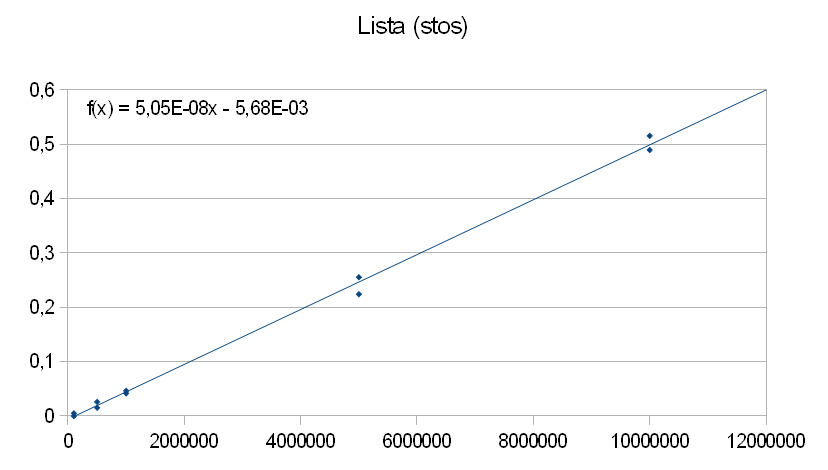
\includegraphics[scale=0.5]{Lista_(stos).png}
\end{center}
\end{figure}

\newpage
\subsection{Kolejka stworzona na podstawie listy}
Klasa odpowiadająca za przechowywanie danych stworzona na podstawie klasy \textit{queue}. 
\begin{center}
\begin {tabular}{|c|c|c|c|c|}\hline
Wielkosc & 1 & 2 & 3 & Średnia \\\hline
100000&0&0&0,016&0,005 \\\hline
100000&0&0&0&0,000 \\\hline
500000&0,016&0,015&0,015&0,015 \\\hline
500000&0,032&0,032&0,031&0,032 \\\hline
1000000&0,031&0,031&0,078&0,047 \\\hline
1000000&0,062&0,031&0,047&0,047 \\\hline
5000000&0,203&0,235&0,219&0,219 \\\hline
5000000&0,25&0,235&0,391&0,292 \\\hline
10000000&0,454&0,547&0,438&0,480 \\\hline
10000000&0,485&0,469&0,953&0,636 \\\hline
\end{tabular}
\end {center}
\begin{figure}[h]
\begin{center}
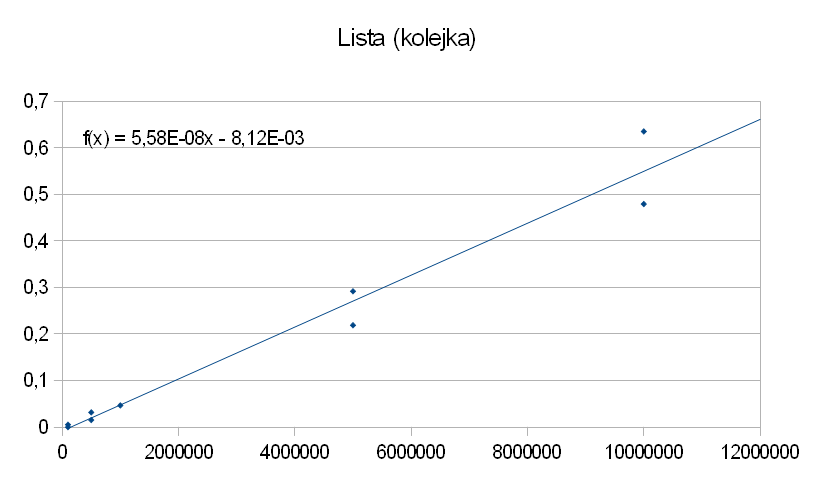
\includegraphics[scale=0.5]{Lista_(kolejka).png}
\end{center}
\end{figure}

\newpage
\section{Wnioski}
Na podstawie danych i wykresów można wyciągnąć następujące wnioski:
\begin{itemize}
\item algorytmy przepisujące tablice za każdym razem mają złożoność obliczeniową o postaci wykładniczej
\item algorytmy podwajające tablice mają złożoność obliczeniową zbliżoną do liniowej
\item z testowanych struktur najszybsze okazały się listy 
\item złożoność obliczeniowa odgrywa duże znaczenie w skuteczności algorytmu
\item różnice czasowe pomiędzy kolejką i stosem są niewielkie
\item zgodnie z oczekiwaniami wartość liczb zapisanych w plikach testowych nie miała wpływu na otrzymywany czas (o ile były to liczby tego samego typu)
\end{itemize}

\end{document}
